\documentclass[../main.tex]{subfiles}

\begin{document}

\chapquote{The beauty of a move lies not in its appearance but in the thought behind it.}{Aron Nimzowitsch}
\chapter{Adapting to new chess sets}
\label{chap:adapting}

Chess sets may vary significantly in appearance. 
As a result, \glspl{cnn} trained on one type of chess set might perform poorly in the inference stage when supplied with images of another chess set. 
This is because we violate the assumption that the training and testing data are drawn from the same distribution.
In light of the theory introduced in \cref{sec:background_transfer_learning}, the natural response is to employ transfer learning in order to fine-tune the \glspl{cnn} to this new data distribution.
Due to the inherent similarities in the data distribution (the fact that they are chess sets and that the source and target tasks are the same), it stands to reason that we could employ a form of \emph{one-shot} transfer learning; 
that is, using only a small amount of data in order to adapt the \glspl{cnn} to the new distribution.
Using the least amount of data necessary will make the system considerably more convenient for the user.

A significant advantage of the chess recognition system as it is developed in \cref{chap:chess_recognition} is the fact that we employ conventional computer vision techniques such as edge and line detection in order to localise the board.
This means that we are able to find the location of practically \emph{any} type of chess board with a high accuracy, not just the board used to generate the training data.
On the other hand, had we employed a board localisation technique based on deep neural networks (for instance a semantic segmentation model), the system would suffer the same type of issues as the \glspl{cnn} mentioned above when required to adapt to new chess sets.
The fact that we can reliably find the corner points of any chess board but may not be able to correctly identify the position on the board gives rise to a system where we could employ transfer learning to obtain better predictions with only minimal extra effort on the part of the user:
if the user wants to employ our system to infer a position on their own chess board, we will instruct them to take a picture of the starting position (\cref{fig:chess_start_position}) from both players' perspectives.
\begin{figure}[h]
    \centering
    \newgame
    \showboard
    \caption[The starting position on the board.]{The starting position on the board. It is the same at the beginning of each game, thus a photo captured in this position is well-suited for transfer learning as the user does not need to manually label the position.}
    \label{fig:chess_start_position}
\end{figure}
The angle of the camera to the chessboard should be in the same interval as used in the data synthesis process depicted in \cref{fig:camera_angle}, i.e. between 45° and 60°.
This chapter will demonstrate how to effectively fine-tune the occupancy and piece classification \glspl{cnn} based on only two input images.

\section{Dataset}
First, we require a dataset in order to evaluate the effectiveness of our approach.
The training set, consisting of the two images obtained in the aforementioned manner is depicted in \cref{fig:transfer_learning_train_data}.
\begin{figure}
    \centering
    \begin{subfigure}[b]{0.47\textwidth}
        \centering
        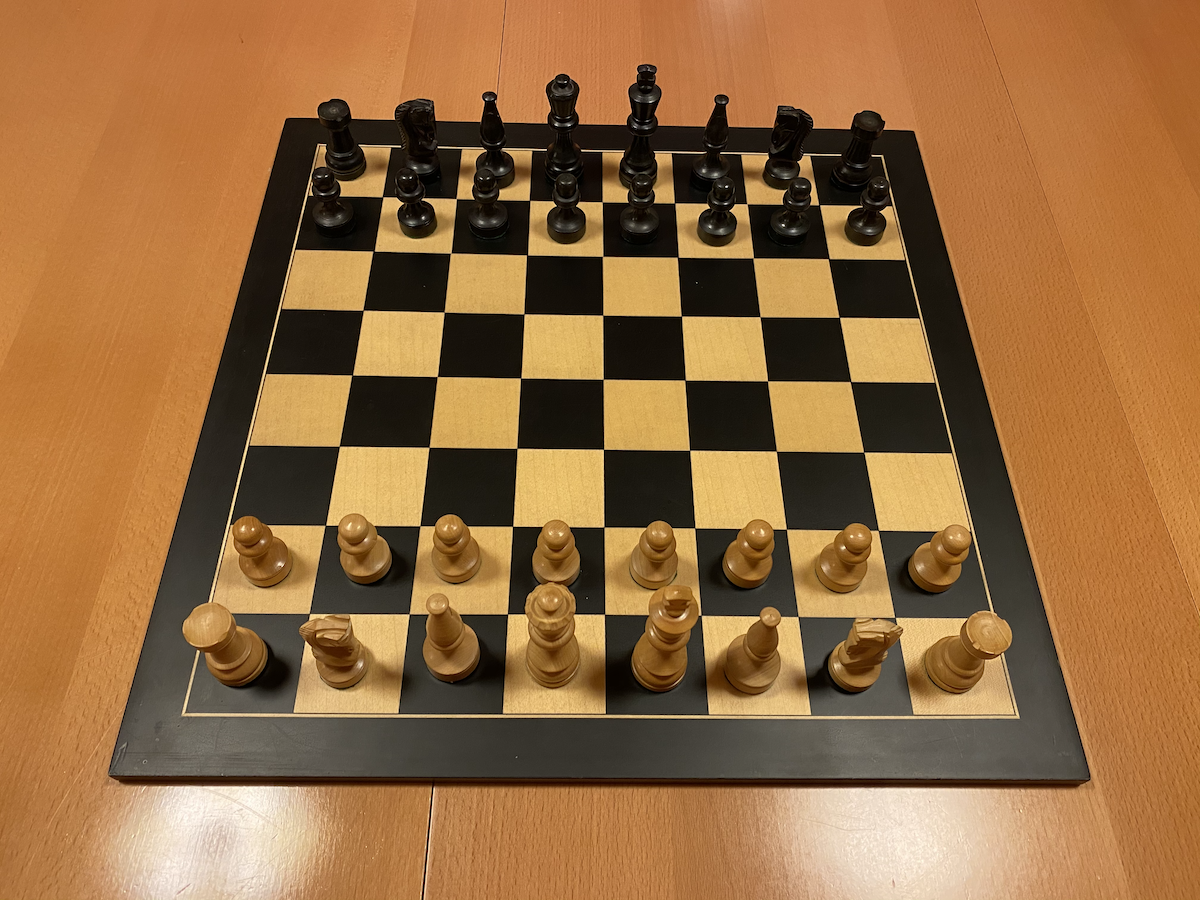
\includegraphics[width=\textwidth]{transfer_learning_white}
        \caption{white player's perspective}
    \end{subfigure}
    \hfill
    \begin{subfigure}[b]{0.47\textwidth}
        \centering
        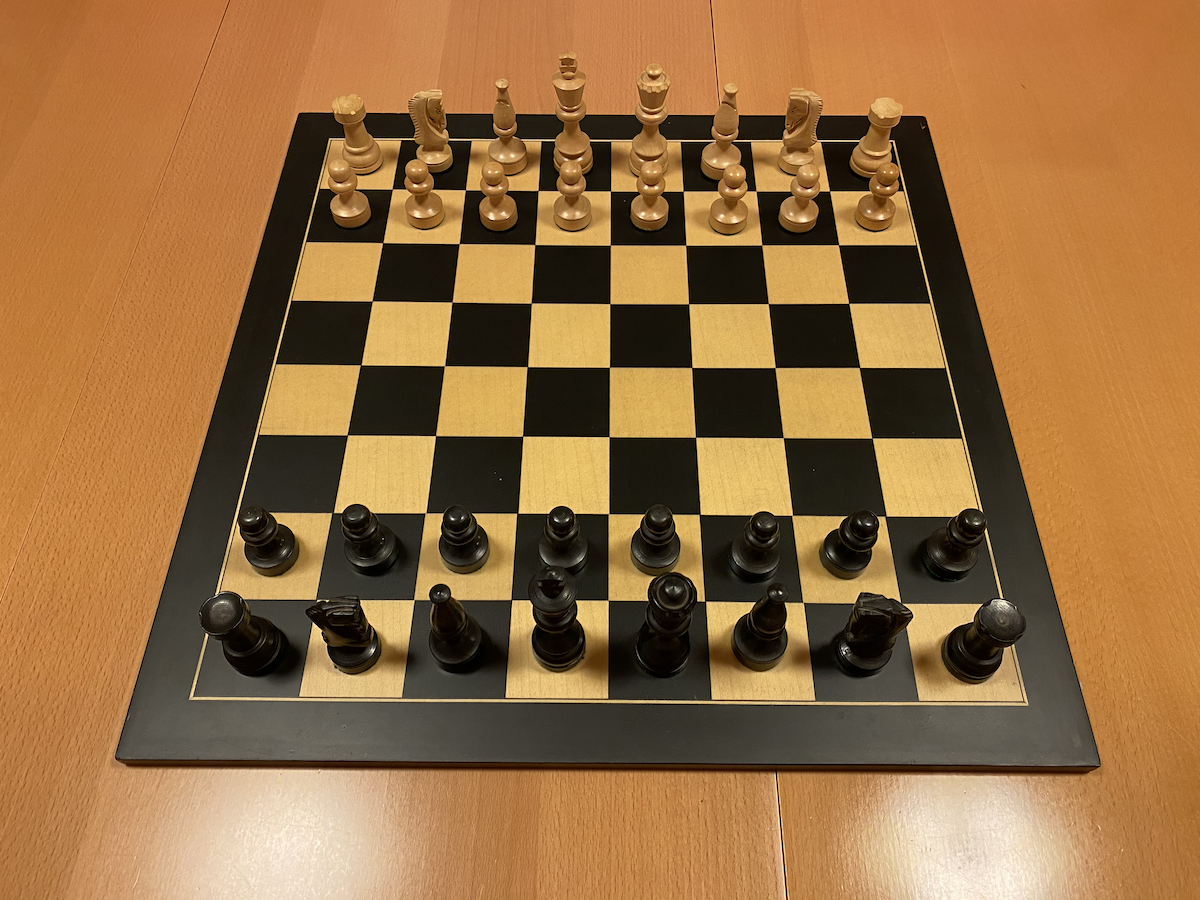
\includegraphics[width=\textwidth]{transfer_learning_black}
        \caption{black player's perspective}
    \end{subfigure}
    \caption{The training dataset used for the transfer learning approach, consisting of only two samples.}
    \label{fig:transfer_learning_train_data}
\end{figure}
For this task, we do not employ a validation dataset because the availability of labelled data is limited (it would be unreasonable to ask the user for more photos and then even requiring them to manually annotate the positions).
The test dataset consists of 27 images which were obtained by playing a game of chess and taking a photo of the board after each move.
Each photo is taken from the current player's perspective, so the images are alternating between White's and Black's perspective.

At this point, it is a good idea to establish a baseline for the quality of predictions the chess recognition pipeline achieves without fine-tuning the \glspl{cnn} on the test set.
\begin{table}
    \centering
    \begin{tabular}{lrr}
        \toprule
        metric & train set & test set \\
        \midrule
        mean number of incorrect squares per board          & 9.50     & 9.33 \\
        per-board end-to-end accuracy                       & 0.00\%   & 0.00\%   \\
        per-board end-to-end accuracy, allowing one mistake & 0.00\%   & 0.00\%   \\
        per-board corner detection accuracy                 & 100.00\% & 100.00\% \\
        per-square occupancy classification accuracy        & 100.00\% & 99.88\% \\
        per-square piece classification accuracy            & 85.16\%  & 85.52\% \\
        \bottomrule
    \end{tabular}
    \caption{Performance of the chess recognition pipeline from \cref{chap:chess_recognition} on the transfer learning dataset without fine-tuning.}
\end{table}
\section{}

\begin{table}
    \centering
    \begin{tabular}{lrr}
        \toprule
        metric & train set & test set \\
        \midrule
        mean number of incorrect squares per board          & 0.00     & 0.11 \\
        per-board end-to-end accuracy                       & 100.00\% & 88.89\%   \\
        per-board end-to-end accuracy, allowing one mistake & 100.00\% & 100.00\%   \\
        per-board corner detection accuracy                 & 100.00\% & 100.00\% \\
        per-square occupancy classification accuracy        & 100.00\% & 99.88\% \\
        per-square piece classification accuracy            & 100.00\% & 99.94\% \\
        \bottomrule
    \end{tabular}
    \caption{Performance of the fine-tuned chess recognition pipeline on the transfer learning dataset.}
\end{table}

\end{document}